\documentclass[12pt, a4paper, notitlepage]{report}
\usepackage{polski}
\usepackage{graphicx}
\usepackage[T1]{fontenc}
\usepackage[utf8]{inputenc}
\usepackage[top=1.5cm, bottom=3cm, left=3cm, right=3cm]{geometry}
\usepackage{amssymb}
\usepackage{tipa}
\usepackage{xcolor}
\makeatletter

\newcommand{\linia}{\rule{\linewidth}{0.4mm}}
\renewcommand{\maketitle}{\begin{titlepage}
	\vspace*{1cm}
	\begin{center}
		\small Fizyka komputerowa\\Wydział Fizyki i Astronomii\\Uniwersytet Wrocławski
	\end{center}
	\vspace{3cm}
	\noindent
	\linia
	\begin{center}
		\LARGE \textsc{\@title}
	\end{center}
	\linia
	\vspace{0.5cm}
	\begin{flushright}
		\begin{minipage}{5cm}
			\textit{\small Autor:}\\ \normalsize \textsc{\@author} \par
		\end{minipage}
		\vspace{5cm}
	\end{flushright}
	\vspace*{\stretch{6}}
	\begin{center}
		\ Styczeń 2021
	\end{center}
\end{titlepage}%
}
\makeatother
\author{Natalia Serwin\\Tomasz Targiel\\Kacper Mordarski}
\title{Zjawisko fotoelektryczne}
\begin{document}
	\maketitle

	\chapter{Fotony}
	\section{Odrobina historii}

	Albert Einstein wykazał, że światło nie tylko jest emitowane porcjami, ale
	rozchodzi się w przestrzeni jako zbiór cząstek – fotonów – i jest pochłaniane
	również porcjami.

	Było to niezwykłe odkrycie, gdyż do tej pory uważano, że światło to fala
	elektromagnetyczna, a wszystkie zjawiska optyczne doskonale wyjaśniała falowa teoria
	światła. Po raz pierwszy pojawiło się w fizyce pojęcie dualizmu
	korpuskularnofalowego. Einstein odkrył korpuskularną\footnote{Korpuskularną =
	cząstkową} naturę światła, wyjaśniając zjawisko fotoelektryczne. Warto
	podkreślić, że za to właśnie odkrycie (a nie za sformułowanie teorii
	względności) Albert Einstein został uhonorowany Nagrodą Nobla.

	\section{Doświadczalne przedstawienie zjawiska fotoelektrycznego}

	\begin{figure}[htp]
		\centering
		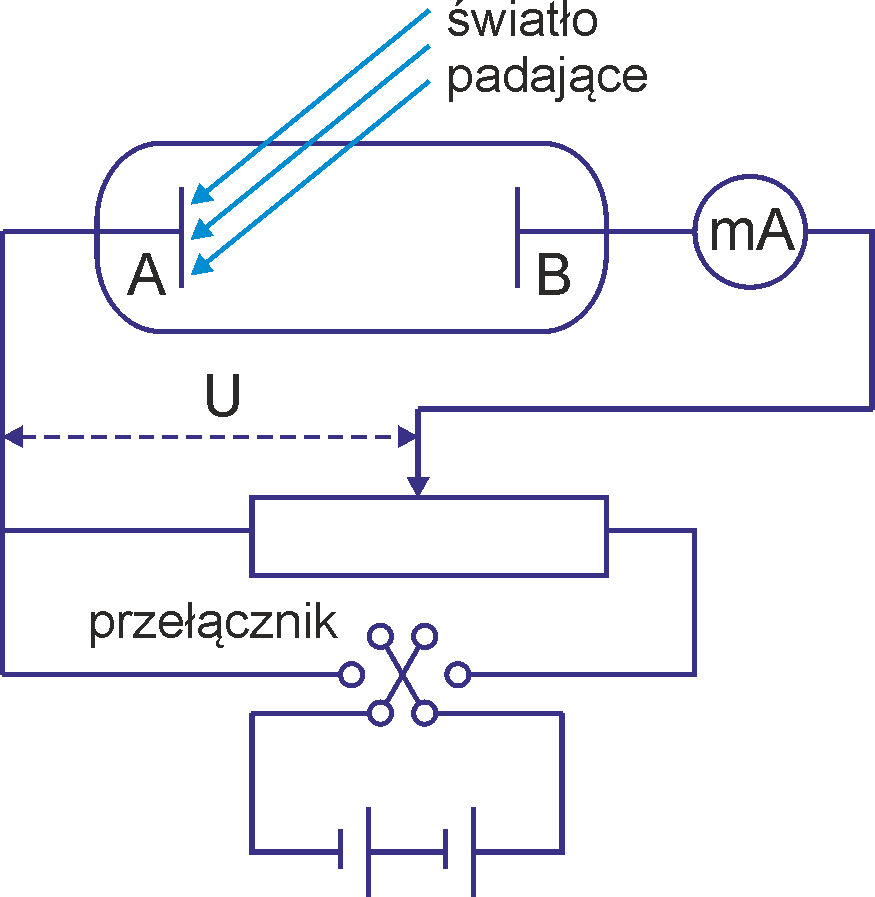
\includegraphics[width=8cm]{img/rysunek_1.1.png}
		\caption{Schemat układu doświadczalnego do badania tego zjawiska}
		\label{fig:1}
	\end{figure}

	W szklanej bańce, w której panuje wysoka próżnia, znajdują się dwie metalowe elektrody
	A i B. Światło pada na metalową płytkę A i uwalnia z niej elektrony, które nazywamy
	fotoelektronami.

	Fotoelektrony są rejestrowane jako prąd elektryczny płynący między płytką A oraz
	elektrodą zbierającą B przy przyłożonym napięciu U. Do pomiaru prądu stosujemy
	czuły miliamperomierz (mA). Poniżej na rysunku pokazana jest zależność prądu fotoelektrycznego
	od przyłożonego napięcia U, dla dwóch różnych wartości natężenia światła.

	\begin{figure}[htp]
		\centering
		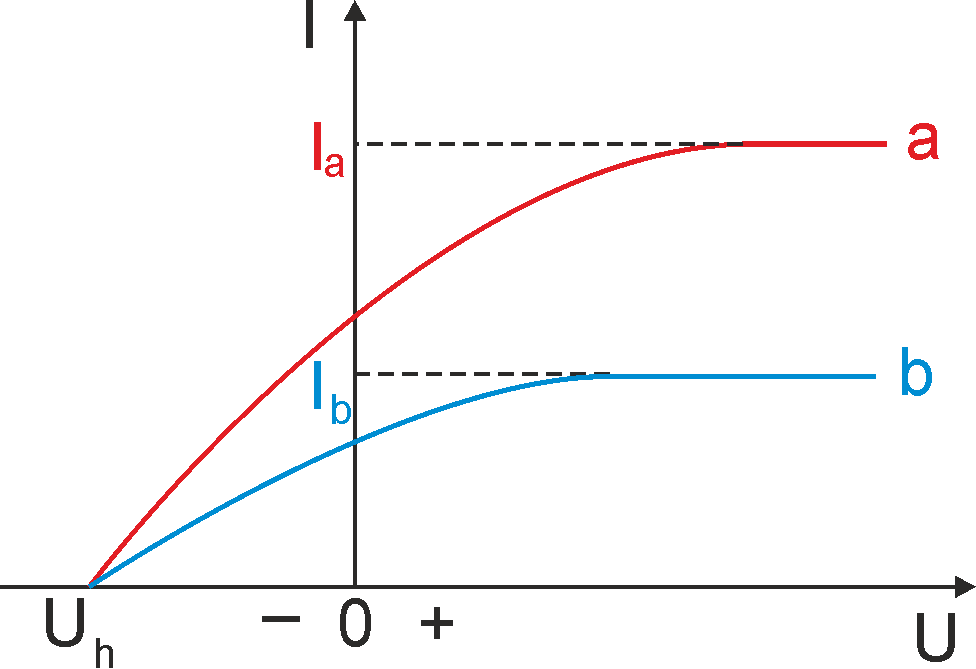
\includegraphics[width=10cm]{img/rysunek_1.2.png}
		\caption{Zależność prądu fotoelektrycznego od przyłożonego napięcia U}
		\label{fig:2}
	\end{figure}

	Widzimy, że gdy napięcie U jest dostatecznie duże, to prąd fotoelektryczny osiąga
	maksymalną wartość (prąd nasycenia Ia, Ib). Odpowiada to sytuacji gdy wszystkie
	elektrony wybijane z płytki A docierają do elektrody B.

	Jeżeli zmienimy znak napięcia U, to prąd nie spada natychmiast do zera (przy U
	= 0 mamy niezerowy prąd). Oznacza to, że fotoelektrony emitowane z płytki A
	mają pewną energię kinetyczną, dzięki której docierają do B (nawet wtedy gdy
	nie są przyspieszane napięciem U).

	Ponadto zauważmy, że nie wszystkie elektrony mają jednakowo dużą energię
	kinetyczną bo tylko część z nich dolatuje do elektrody B; przy U = 0 prąd jest
	mniejszy od maksymalnego. Wreszcie przy dostatecznie dużym napięciu równym Uh
	zwanym napięciem hamowania prąd zanika. Różnica potencjałów Uh pomnożona przez
	ładunek elektronu e jest więc miarą energii najszybszych elektronów (przy U =
	Uh nawet najszybsze elektrony są zahamowane, nie dochodzą do elektrody B.

	\begin{equation}
		E_{kmax}=eU_{h}
	\end{equation}

	Krzywe na rysunku 1.2 różnią się natężeniem padającego światła. Przy silniejszym
	oświetleniu {\color{red}(krzywa a)} otrzymujemy większy prąd nasycenia ale takie
	samo napięcie hamowania jak dla układu oświetlonego słabiej {\color{blue}(krzywa b)}.

	Widać więc, że $E_{kmax}$ nie zależy od natężenia światła. Zmienia się tylko prąd
	nasycenia, a to oznacza, że wiązka światła o większym natężeniu wybija więcej elektronów,
	ale nie szybszych.

	Wynik innego doświadczenia pokazuje rysunek 1.3. Wykreślono tu zależność napięcia
	hamowania od częstotliwości (barwy) światła padającego na powierzchnie sodu metalicznego.
	Zauważmy, że otrzymano zależność liniową oraz że istnieje pewna wartość progowa
	częstotliwości v0 , poniżej której zjawisko fotoelektryczne nie występuje.

	\begin{figure}[htp]
		\centering
		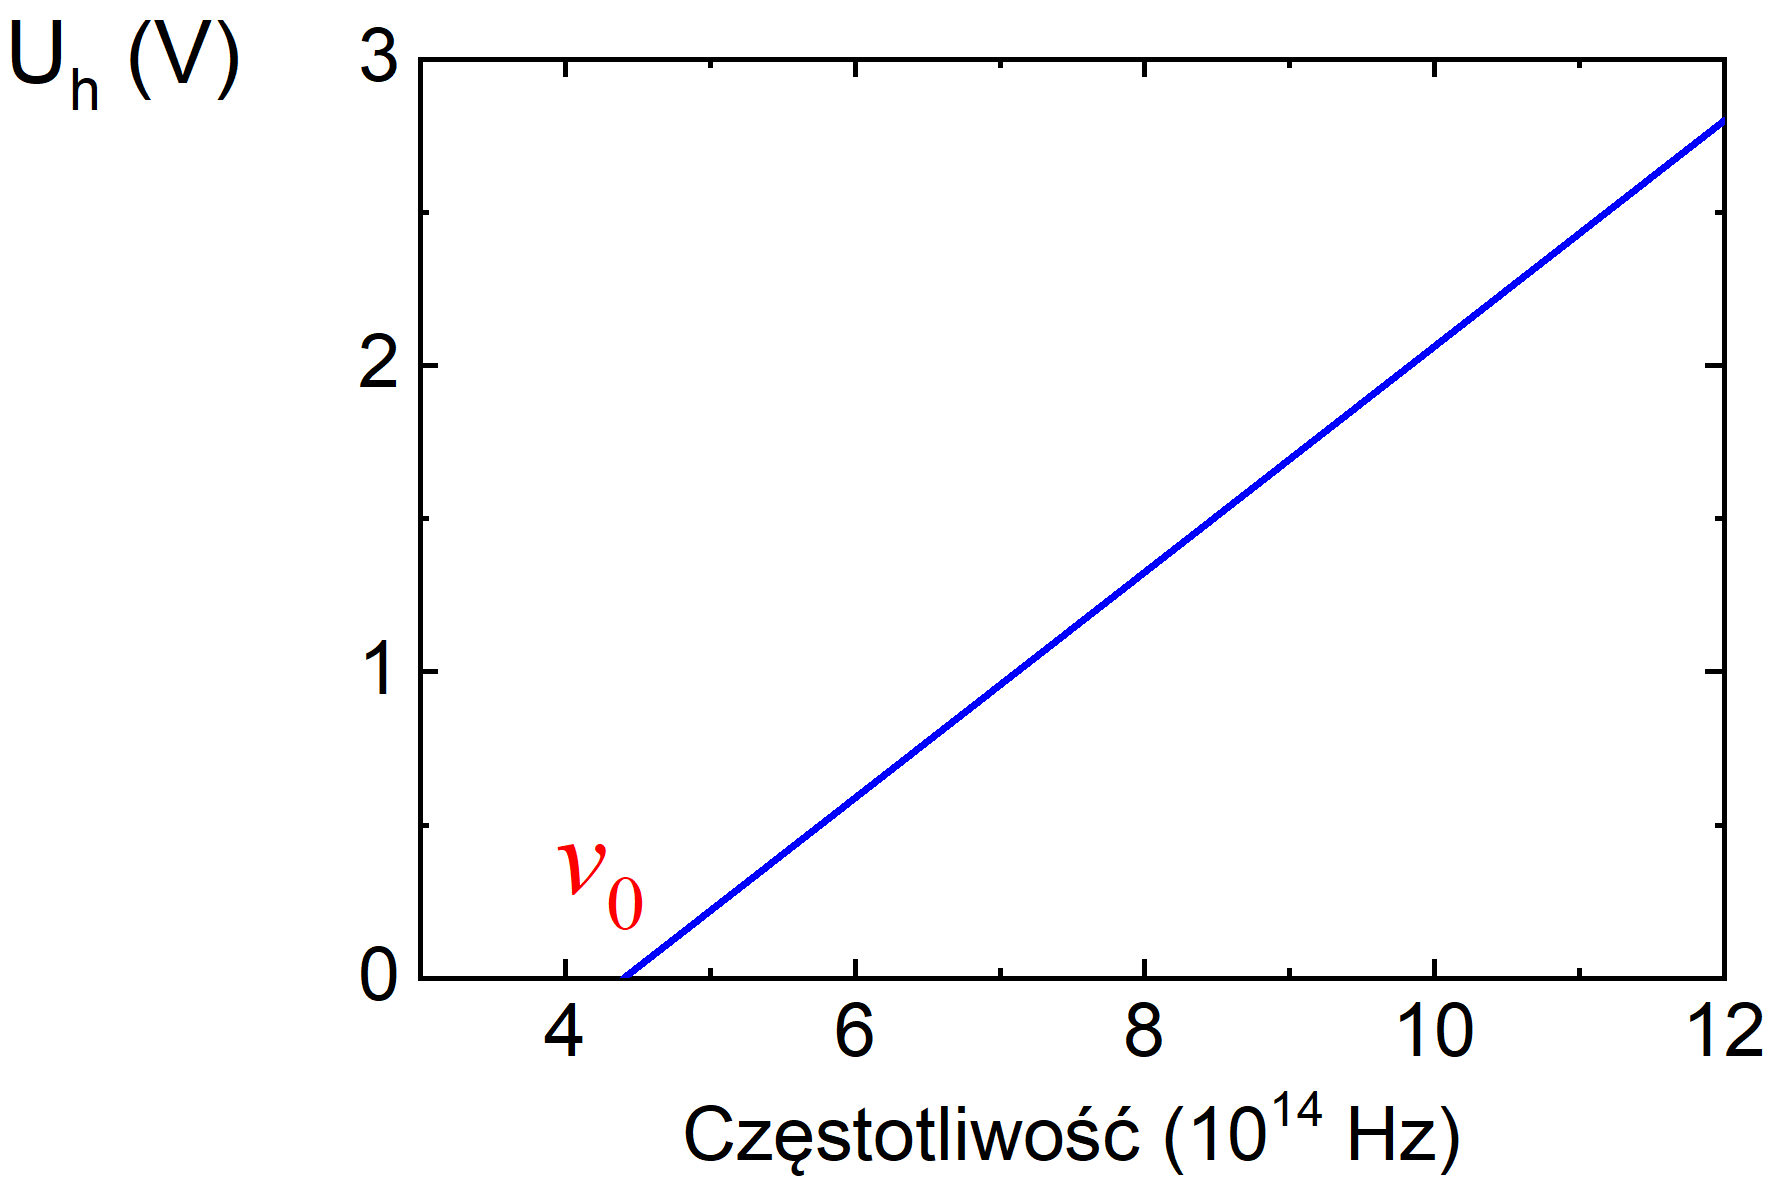
\includegraphics[width=8cm]{img/rysunek_1.3.png}
		\caption{Zależność napięcia hamowania od częstotliwości światła dla sodu}
		\label{fig:3}
	\end{figure}

	\section{Cechy efektu fotoelektrycznego}

	Efekt fotoelektryczny ma trzy istotne cechy, których nie da się wytłumaczyć w
	ramach fizyki klasycznej: brak opóźnienia, niezależność energii kinetycznej
	fotoelektronów od natężenia padającego promieniowania oraz występowanie
	częstotliwości granicznej.

	\subsection{Brak opóźnienia}

	Gdy promieniowanie pada na metalową płytkę elektrody, elektrony emitowane są
	natychmiast, nawet przy bardzo niewielkim natężeniu promieniowania. Brak
	opóźnienia stoi w sprzeczności z klasyczną fizyką, w ramach której przewiduje się,
	że zwłaszcza przy niskim natężeniu padającego światła powinno minąć nieco
	czasu, zanim elektrony pobiorą wystarczającą ilość energii, aby uwolnić się z
	powierzchni metalu. Takie opóźnienie nie jest jednak obserwowane.

	\subsection{Natężenie padającego promieniowania, a energia kinetyczna elektronów}

	Typowe krzywe eksperymentalne pokazane są na rysunku 1.2. Przy dodatniej różnicy
	potencjałów natężenie stopniowo rośnie aż do uzyskania pewniej wartości.
	Dalsze zwiększanie napięcia nie powoduje wzrostu natężenia. Wyższe natężenie padającego
	promieniowania pociąga za sobą większe natężenie fotoprądu. Gdy różnica
	potencjałów jest ujemna, wzrost jej wartości absolutnej powoduje, że wartość
	natężenia prądu spada, aż osiąga zero przy napięciu hamowania. Wartość tego
	napięcia nie zależy od natężenia padającego promieniowania.

	Aby zrozumieć, dlaczego tego rezultatu nie da się wytłumaczyć na gruncie fizyki
	klasycznej, rozważmy wpierw energię fotoelektronów. Opuszczający powierzchnię płytki
	fotoelektron ma energię kinetyczną $E_{k0}$, którą uzyskał od padającego
	promieniowania. W przestrzeni pomiędzy elektrodami elektron porusza się w polu
	elektrostatycznym, a jego energia potencjalna zmienia się o $q\Delta V$, gdzie
	$\Delta V$ jest różnicą potencjałów, a q=-e. Z zasady zachowania energii
	wynika więc, że $\Delta E_{k}-e\Delta V=0J$ ($\Delta E_{k}$ jest zmianą
	energii kinetyczej fotoelektronu). Gdy przyłożymy napięcie hamowania
	$-\Delta V_{h}$ , fotoelektron traci całą swoją energię kinetyczną $E_{ki}$ i
	zatrzymuje się. Bilans energetyczny wyraża się wtedy następująco:
	$(0J-E_{k0})-e(-\Delta V_{h})=0J$, z czego wynika, że $E_{k0}=e\Delta V_{h}$. Napięcie
	hamowania pozwala nam więc wyznaczyć maksymalną energie kinetyczną $E_{kmax}$ emitowanych
	elektronów

	\begin{equation}
		E_{kmax}=e\Delta V_{h}
	\end{equation}

	Korzystając z tego wyniku, możemy zrozumieć, dlaczego mechanika klasyczna nie tłumaczy
	nam wyników eksperymentu. W teorii klasycznej fotoelektron absorbuje energię w
	sposób ciągły, oznacza to, że gdy padające promieniowanie ma duże natężenie, energia
	kinetyczna także powinna być duża. Podobnie w przypadku niskiego natężenia
	promieniowania energia kinetyczna wybitych fotoelektronów powinna być mała. Eksperyment
	wskazuje jednak, że napięcie hamowania, a więc i maksymalna wartość energii kinetycznej
	fotoelektronów nie zależą od natężenia światła.

	\subsection{Częstotliwość progowa}

	Dla każdej metalowej powierzchni, na którą pada promieniowanie, istnieje pewna
	częstotliwość tego promieniowania, poniżej której nie rejestruje się fotoprądu
	– innymi słowy zjawisko fotoelektryczne nie zachodzi. Wielkość taką nazywamy
	częstotliwością progową (ang. cut-off frequency) i jest ona charakterystyczna dla
	danego metalu. Dane eksperymentalne pokazują liniową zależność – maksymalna
	energia kinetyczna fotoelektronów rośnie liniowo ze zwiększającą się
	częstotliwością podającego promieniowania. Pomiary dokonywane dla różnych metali
	dają liniową zależność z tym samym nachyleniem wykresu. Żadna z tych
	obserwacji nie daje się pogodzić z fizyką klasyczną, w ramach której energia kinetyczna
	fotoelektronów nie powinna zależeć od częstotliwości, ale od natężenia
	padającego światła. Fizyka klasyczna nie przewiduje także istnienia częstotliwości
	progowej. Ponieważ w klasycznym obrazie elektrony pobierają energię od
	promieniowania w sposób ciągły, ich energia kinetyczna powinna zależeć tylko od
	natężenia padającego światła, a efekt powinien zachodzić zawsze, niezależnie od
	częstotliwości.

	\begin{figure}[htp]
		\centering
		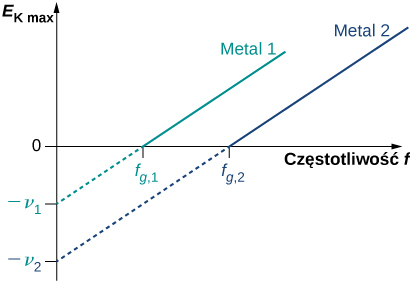
\includegraphics[width=8cm]{img/rysunek_1.4.jpeg}
		\caption{Liniowy wzrost energii kinetycznej ze zwiększającą się
		częstotliwością podającego promieniowania}
		\label{fig:4}
	\end{figure}

	\section{Kwantowa teoria Einsteina zjawiska fotoelektrycznego}
	Efekt fotoelektryczny został wyjaśniony w 1905 roku przez Alberta Einsteina. Założył
	on, że skoro hipoteza Plancka o kwantach energii poprawnie opisywała wymianę
	energii między promieniowaniem elektromagnetycznym i ścianami wnęki, to powinna
	być ona także zastosowana do opisu absorpcji promieniowania przez fotoelektrodę.
	Zapostulował on tezę, że fala elektromagnetyczna niesie energię w dyskretnych porcjach.
	Einstein rozszerzył hipotezę Plancka, postulując, że samo światło składa się z
	kwantów promieniowania. Innymi słowy, że fale elektromagnetyczne są
	skwantowane.

	W podejściu Einsteina wiązka monochromatycznego światła o częstotliwości
	$\mathcal{V}$ złożona jest z fotonów, czyli foton jest cząstką światła. Każdy
	foton porusza się z prędkością światła i niesie kwant energii $E_{f}$. Energia
	fotonów zależy tylko od częstotliwości $\mathcal{V}$ i dana jest wzorem

	\begin{equation}
		E_{f}=h \mathcal{V}
	\end{equation}

	gdzie h jest stałą Plancka.

	W efekcie fotoelektrycznym fotony docierają do metalowej powierzchni i każdy foton
	oddaje całą swoją energię tylko jednemu elektronowi. To zjawisko kwantowe stoi
	w sprzeczności z mechaniką klasyczną, według której wymiana energii zachodzi w
	sposób ciągły. Bilans energetyczny elektronu, który przejmuje od fotonu pewną energię
	$E_{f}$, jest następujący

	\begin{equation}
		E_{f}=E_{kmax}+W
	\end{equation}

	Równanie to jest bardzo proste, ma jednak głebokie znacznie.

	W interpretacji Einsteina oddziaływania zachodzą pomiędzy pojedynczymi elektronami
	i fotonami. Brak opóźnienia świadczy o tym, że to oddziaływanie zachodzi natychmiast.
	Czasu oddziaływania nie da się zwiększyć, zmniejszając natężenie padającego światła.
	Natężenie światła odpowiada liczbie fotonów padających na powierzchnię metalu
	w jednostce czasu. Nawet przy bardzo małych wartościach natężenia efekt fotoelektryczny
	wciąż występuje, gdyż oddziaływanie zachodzi pomiędzy jednym elektronem i
	jednym fotonem. Tak długo, jak pada chociaż jeden foton z wystarczająco dużą
	energią, aby wybić z metalu elektron, tak długo zjawisko elektryczne będzie
	zachodziło.

	Występowanie częstotliwości progowej $\mathcal{V}_{g}$ w efekcie
	fotoelektrycznym bezpośrednio wynika z równania 1.4, ponieważ energia kinetyczna
	$E_{kmax}$ fotoelektronu może przyjmować tylko wartości dodatnie. Oznacza to, że
	istnieje taka częstotliwość, dla której energia ta wynosi zero, $0J=h\mathcal{V}
	_{g} -W$. Jest to właśnie częstotliwość progowa

	\begin{equation}
		\mathcal{V}_{g} =\frac{W}{h}
	\end{equation}

	Częstotliwość progowa zależy tylko od pracy wyjścia danego metalu i jest do
	niej wprost proporcjonalna. Gdy praca wyjścia jest duża (elektrony są mocno
	związane w metalu), energia progowa fotonu musi być wystarczająca, by wybić fotoelektron,
	co odpowiada dużej częstotliwości. Fotony o częstotliwości większej od częstotliwości
	progowej $\mathcal{V}_{g}$ wybijają elektrony, gdyż $E_{kmax}>0J$. Fotony o częstotliwościach
	mniejszych niż $\mathcal{V}_{g}$ nie mają wystarczającej energii, by wybić
	fotoelektrony. W związku z tym, gdy padające promieniowanie ma częstotliwość
	niższą od progowej, efekt fotoelektryczny nie zachodzi. Ponieważ częstotliwość
	$\mathcal{V}$ i długość fali $\lambda$ fal elektromagnetycznych są ze sobą
	powiązane $\lambda \mathcal{V}=c$ (gdzie c jest prędkością światła w próżni), częstotliwości
	progowej odpowiada progowa długość fali $\lambda_{0}$.

	\begin{equation}
		\lambda_{0} =\frac{c}{\mathcal{V}_{g}}=\frac{c}{W/h}=\frac{hc}{W}
	\end{equation}

	gdzie $h_{c}=1240eVnm$. Obserwacje nasze możemy przeformułować w następujący sposób:
	gdy padające promieniowanie ma długość fali większą od długości progowej, efekt
	fotoelektryczny nie zachodzi.

	\begin{thebibliography}{99}
		\bibitem{1} R. Resnick, D. Halliday: \emph{Podstawy fizyki}, Wyd. 7 T. 2. Warszawa:
			Wydawnictwo Naukowe PWN, 1993. ISBN 83-01-09324-2

		\bibitem{2} I.W. Sawieliew: \emph{Wykłady z fizyki 3.}, Wyd. 2 Warszawa: Wydawnictwo
			Naukowe PWN, 1994. ISBN 83-01-11606-4

		\bibitem{3} B. Średniawa:: \emph{Mechanika kwantowa}, Warszawa: Państwowe Wydawnictwo
			Naukowe, 1978
	\end{thebibliography}
\end{document}